\hintsection{\Cref*{chGettingStarted}}

Before we can start proving things, we need to eliminate certain kinds of statements that we might try to prove. Consider the following statement:
\begin{center} \textit{This sentence is false.} \end{center}
Is it true or false? If you think about this for a couple of seconds then you'll get into a bit of a pickle.

Now consider the following statement:
\begin{center} \textit{The happiest donkey in the world.} \end{center}
Is it true or false? Well it's not even a sentence; it doesn't make sense to even \textit{ask} if it's true or false!

Clearly we'll be wasting our time trying to write proofs of statements like the two listed above---we need to narrow our scope to statements that we might actually have a chance of proving (or perhaps refuting)! This motivates the following (informal) definition.

\begin{definition}
\label{defProposition}
\label{defProof}
\index{proposition}
\index{proof}
A \textbf{proposition} \index{proposition} is a statement to which it is possible to assign a \textbf{truth value} (`true' or `false'). If a proposition is true, a \textbf{proof} of the proposition is a logically valid argument demonstrating that it is true, which is pitched at such a level that a member of the intended audience can verify its correctness.
\end{definition}

Thus the statements given above are not propositions because there is no possible way of assigning them a truth value. Note that, in \Cref{defProposition}, all that matters is that it \textit{makes sense} to say that it is true or false, regardless of whether it actually \textit{is} true or false---the truth value of many propositions is unknown, even very simple ones.

\begin{exercise}
Think of an example of a true proposition, a false proposition, a proposition whose truth value you don't know, and a statement that is not a proposition.
\end{exercise}

Results in mathematical papers and textbooks may be referred to as \textit{propositions}, but they may also be referred to as \textit{theorems}, \textit{lemmas} or \textit{corollaries} depending on their intended usage.
\begin{itemize} 
\item A \textbf{proposition} is an umbrella term which can be used for any result.
\item A \textbf{theorem} is a key result which is particularly important.
\item A \textbf{lemma} is a result which is proved for the purposes of being used in the proof of a theorem. 
\item A \textbf{corollary} is a result which follows from a theorem without much additional effort.
\end{itemize}
These are not precise definitions, and they are not meant to be---you could call every result a \textit{proposition} if you wanted to---but using these words appropriately helps readers work out how to read a paper. For example, if you just want to skim a paper and find its key results, you'd look for results labelled as \textit{theorems}.

It is not much good trying to prove results if we don't have anything to prove results about. With this in mind, we will now introduce the \textit{number sets} and prove some results about them in the context of four topics, namely: division of integers, number bases, rational and irrational numbers, and polynomials. These topics will provide context for the material in \Cref{ptCoreConcepts}, and serve as an introduction to the topics covered in \Cref{ptTopics}.

We will not go into very much depth in this chapter. Rather, think of this as a warm-up exercise---a quick, light introduction, with more proofs to be provided in the rest of the book.

\subsection*{Number sets}

Later in this chapter, and then in much more detail in \Cref{chSets}, we will encounter the notion of a \textit{set}; a set can be thought of as being a collection of objects. This seemingly simple notion is fundamental to mathematics, and is so involved that we will not treat sets formally in this book. For now, the following definition will suffice.

\begin{definition}[to be revised in \Cref{defSet}]
\label{defSetsPreliminary}
\lindexmmc{in}{$\in$}
A \textbf{set} is a collection of objects. The objects in the set are called \textbf{elements} of the set. If $X$ is a set and $x$ is an object, then we write $x \in X$ \inlatexnb{x \textbackslash{}in X} to denote the assertion that $x$ is an element of $X$.
\end{definition}

The sets of concern to us first and foremost are the \textit{number sets}---that is, sets whose elements are particular types of \textit{number}. At this introductory level, many details will be temporarily swept under the rug; we will work at a level of precision which is appropriate for our current stage, but still allows us to develop a reasonable amount of intuition.

In order to define the number sets, we will need three things: an infinite line, a fixed point on this line, and a fixed unit of length.

So here we go. Here is an infinite line:
\begin{center}
\begin{tikzpicture}
\draw[latex-latex] (-5.5, 0) -- (5.5, 0) ;
\end{tikzpicture}
\end{center}
The arrows indicate that it is supposed to extend in both directions without end. The points on the line will represent numbers (specifically, \textit{real numbers}, a misleading term that will be defined in \Cref{defRealsInformal}). Now let's fix a point on this line, and label it `$0$':
\begin{center}
\begin{tikzpicture}
\draw[latex-latex] (-5.5, 0) -- (5.5, 0) ; 
\draw (0, 0) -- (0, 0.1) node[above] {$0$} ;
\end{tikzpicture}
\end{center}
This point can be thought of as representing the number zero; it is the point against which all other numbers will be measured. Finally, let's fix a unit of length:
\begin{center}
\begin{tikzpicture}
\draw (0, 0) -- (1, 0) ; 
\foreach \x in {0,1} \draw (\x, -0.1) -- (\x, 0.1)  ;
\end{tikzpicture}
\end{center}
This unit of length will be used, amongst other things, to compare the extent to which the other numbers differ from zero.

\begin{definition}
\label{defNumberLine}
The above infinite line, together with its fixed zero point and fixed unit length, constitute the (\textbf{real}) \textbf{number line}.
\end{definition}

We will use the number line to construct five sets of numbers of interest to us:
\begin{itemize}
\item The set $\mathbb{N}$ of \textit{natural numbers}---\Cref{defNaturalNumbersInformal};
\item The set $\mathbb{Z}$ of \textit{integers}---\Cref{defIntegersInformal};
\item The set $\mathbb{Q}$ of \textit{rational numbers}---\Cref{defRationalsInformal};
\item The set $\mathbb{R}$ of \textit{real numbers}---\Cref{defRealsInformal}; and
\item The set $\mathbb{C}$ of \textit{complex numbers}---\Cref{defComplexNumbersInformal}.
\end{itemize}

Each of these sets has a different character and is used for different purposes, as we will see both later in this chapter and throughout this book.

\subsection*{Natural numbers ($\mathbb{N}$)}

The \textit{natural numbers} are the numbers used for counting---they are the answers to questions of the form `how many'---for example, I have \textit{three} uncles, \textit{one} dog and \textit{zero} cats.

Counting is a skill humans have had for a very long time; we know this because there is evidence of people using tally marks tens of thousands of years ago. Tally marks provide one method of counting small numbers: starting with nothing, proceed through the objects you want to count one by one, and make a mark for every object. When you are finished, there will be as many marks as there are objects. We are taught from a young age to count with our fingers; this is another instance of making tally marks, where now instead of making a mark we raise a finger.

Making a tally mark represents an \textit{increment} in quantity---that is, adding one. On our number line, we can represent an increment in quantity by moving to the right by the unit length. Then the distance from zero we have moved, which is equal to the number of times we moved right by the unit length, is therefore equal to the number of objects being counted.

\begin{definition}
\label{defNaturalNumbersInformal}
The \textbf{natural numbers} are represented by the points on the number line which can be obtained by starting at $0$ and moving right by the unit length any number of times:
\begin{center}
\begin{tikzpicture}
\draw[latex-latex] (-5.5, 0) -- (5.5, 0) ; 
\foreach \x in {0,1,2,3,4,5} \draw (\x, 0) -- (\x, 0.1) node[above] {$\x$} ;
\end{tikzpicture}
\end{center}
In more familiar terms, they are the \textit{non-negative whole numbers}. We write $\mathbb{N}$ \inlatex{mathbb\{N\}}\lindexmmc{mathbb}{$\mathbb{A}, \mathbb{B}, \dots$} for the set of all natural numbers; thus, the notation `$n \in \mathbb{N}$' means that $n$ is a natural number.
\end{definition}

The natural numbers have very important and interesting mathematical structure, and are central to the material in \Cref{chCombinatorics}. A more precise characterisation of the natural numbers will be provided in \Cref{secPeanosAxioms}, and a mathematical construction of the set of natural numbers can be found in \Cref{secZFC} (see \Cref{cnsNaturalNumbersVonNeumann}). Central to these more precise characterisations will be the notions of `zero' and of `adding one'---just like making tally marks.

\begin{aside}
Some authors define the natural numbers to be the \textit{positive} whole numbers, thus excluding zero. We take $0$ to be a natural number since our main use of the natural numbers will be for counting finite sets, and a set with nothing in it is certainly finite! That said, as with any mathematical definition, the choice about whether $0 \in \mathbb{N}$ or $0 \not \in \mathbb{N}$ is a matter of taste or convenience, and is merely a convention---it is not something that can be proved or refuted.
\end{aside}

\subsection*{Number bases}

Writing numbers down is something that may seem easy to you now, but it likely took you several years as a child to truly understand what was going on. Historically, there have been many different systems for representing numbers symbolically, called \textit{numeral systems}.\index{numeral system} First came the most primitive of all, tally marks, appearing in the Stone Age and still being used for some purposes today. Thousands of years and hundreds of numeral systems later, there is one dominant numeral system, understood throughout the world: the \textbf{Hindu--Arabic numeral system}.\index{numeral system!Hindu--Arabic} This numeral system consists of ten symbols, called \textit{digits}. It is a \textit{positional} numeral system, meaning that the position of a symbol in a string determines its numerical value.

In English, the \textit{Arabic numerals} are used as the ten digits:
\[ 0 \quad 1 \quad 2 \quad 3 \quad 4 \quad 5 \quad 6 \quad 7 \quad 8 \quad 9 \]
The right-most digit in a string is in the units place, and the value of each digit increases by a factor of ten moving to the left. For example, when we write `$2812$', the left-most `$2$' represents the number two thousand, whereas the last `$2$' represents the number two.

The fact that there are ten digits, and that the numeral system is based on powers of ten, is a biological accident corresponding with the fact that most humans have ten fingers. For many purposes, this is inconvenient. For example, ten does not have many positive divisors (only four)---this has implications for the ease of performing arithmetic; a system based on the number twelve, which has six positive divisors, might be more convenient. Another example is in computing and digital electronics, where it is more convenient to work in a \textit{binary} system, with just two digits, which represent `off' and `on' (or `low voltage' and `high voltage'), respectively; arithmetic can then be performed directly using sequences of \textit{logic gates} in an electrical circuit.

It is therefore worthwhile to have some understanding of positional numeral systems based on numbers other than ten. The mathematical abstraction we make leads to the definition of \textit{base-$b$ expansion}.

\begin{definition}
\label{defBaseBExpansionPreliminary}
\index{base-$b$ expansion}
\index{number base}
Let $b>1$. The \textbf{base-$b$ expansion} of a natural number $n$ is the\footnote{The use of the word `the' is troublesome here, since it assumes that every natural number has only one base-$b$ expansion. This fact actually requires proof---see \Cref{thmBaseBExpansion}.} string $d_r d_{r-1} \dots d_0$ such that
\begin{itemize}
\item $n = d_r \cdot b^r + d_{r-1} \cdot b^{r-1} + \cdots + d_0 \cdot b^0$;
\item $0 \le d_i < b$ for each $i$; and
\item If $n>0$ then $d_r \ne 0$---the base-$b$ expansion of zero is $0$ in all bases $b$.
\end{itemize}
Certain number bases have names; for instance, the base-$2$, $3$, $8$, $10$ and $16$ expansions are respectively called \textit{binary}, \textit{ternary}, \textit{octal}, \textit{decimal} and \textit{hexadecimal}.
\end{definition}

\begin{example}
Consider the number $1023$. Its decimal (base-$10$) expansion is $1023$, since
\[ 1023 = 1 \cdot 10^3 + 0 \cdot 10^2 + 2 \cdot 10^1 + 3 \cdot 10^0 \]
Its binary (base-$2$) expansion is $1111111111$, since
\[ 1023 = 1 \cdot 2^9 + 1 \cdot 2^8 + 1 \cdot 2^7 + 1 \cdot 2^6 + 1 \cdot 2^5 + 1 \cdot 2^4 + 1 \cdot 2^3 + 1 \cdot 2^2 + 1 \cdot 2^1 + 1 \cdot 2^0 \]
We can express numbers in base-$36$ by using the ten usual digits $0$ through $9$ and the twenty-six letters $\mathrm{A}$ through $\mathrm{Z}$; for instance, $\mathrm{A}$ represents $10$, $\mathrm{M}$ represents $22$ and $\mathrm{Z}$ represents $35$. The base-$36$ expansion of $1023$ is $\mathrm{SF}$, since
\[ 1023 = 28 \cdot 36^1 + 15 \cdot 36^0 = \mathrm{S} \cdot 36^1 + \mathrm{F} \cdot 36^0 \]
\end{example}

\begin{exercise}
Find the binary, ternary, octal, decimal, hexadecimal and base-$36$ expansions of the number $21127$, using the letters $\mathrm{A}$--$\mathrm{F}$ as additional digits for the hexadecimal expansion and the letters $\mathrm{A}$--$\mathrm{Z}$ as additional digits for the base-$36$ expansion.
\end{exercise}

We sometimes wish to specify a natural number in terms of its base-$b$ expansion; we have some notation for this.

\begin{notation}
Let $b>1$. If the numbers $d_0,d_1,\dots,d_r$ are base-$b$ digits (in the sense of \Cref{defBaseBExpansionPreliminary}), then we write
\[ {d_rd_{r-1} \dots d_0}_{(b)} = d_r \cdot b^r + d_{r-1} \cdot b^{r-1} + \cdots + d_0 \cdot b^0 \]
for the natural number whose base-$b$ expansion is $d_rd_{r-1} \dots d_0$. If there is no subscript $(b)$ and a base is not specified explicitly, the expansion will be assumed to be in base-$10$.
\end{notation}

\begin{example}
Using our new notation, we have
\[ 1023 = 1111111111_{(2)} = 1101220_{(3)} = 1777_{(8)} = 1023_{(10)} = 3\mathrm{FF}_{(16)} = \mathrm{SF}_{(36)} \]
\end{example}

\subsection*{Integers ($\mathbb{Z}$)}

The \textit{integers} can be used for measuring the difference between two instances of counting. For example, suppose I have five apples and five bananas. Another person, also holding apples and bananas, wishes to trade. After our exchange, I have seven apples and only one banana. Thus I have two more apples and four fewer bananas.

Since an increment in quantity can be represented by moving to the right on the number line by the unit length, a \textit{decrement} in quantity can therefore be represented by moving to the \textit{left} by the unit length. Doing so gives rise to the integers.

\begin{definition}
\label{defIntegersInformal}
The \textbf{integers} are represented by the points on the number line which can be obtained by starting at $0$ and moving in either direction by the unit length any number of times:
\begin{center}
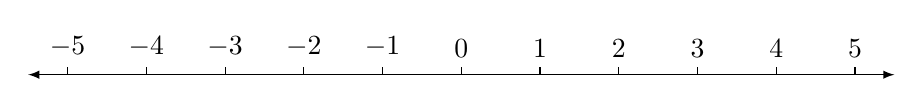
\begin{tikzpicture}
\draw[latex-latex] (-5.5, 0) -- (5.5, 0) ; 
\foreach \x in {-5,-4,-3,-2,-1,0,1,2,3,4,5} \draw (\x, 0) -- (\x, 0.1) node[above] {$\x$} ;
\end{tikzpicture}
\end{center}
We write $\mathbb{Z}$ \inlatex{mathbb\{Z\}}\lindexmmc{mathbb}{$\mathbb{A}, \mathbb{B}, \dots$} for the set of all integers; thus, the notation `$n \in \mathbb{Z}$' means that $n$ is an integer.
\end{definition}

The integers have such a fascinating structure that a whole chapter of this book is devoted to them---see \Cref{chNumberTheory}. This is to do with the fact that, although you can add, subtract and multiply two integers and obtain another integer, the same is not true of division. This `bad behaviour' of division is what makes the integers interesting. We will now see some basic results about division.

\subsection*{Division of integers}
\label{pGettingStartedDivision}

The motivation we will soon give for the definition of the rational numbers (\Cref{defRationalsInformal}) is that the result of dividing one integer by another integer is not necessarily another integer. However, the result is \textit{sometimes} another integer; for example, I can divide six apples between three people, and each person will receive an integral number of apples. This makes division interesting: how can we measure the failure of one integer's divisibility by another? How can we deduce when one integer is divisible by another? What is the structure of the set of integers when viewed through the lens of division? This motivates \Cref{defDivisionPreliminary}.

\begin{definition}[to be repeated in \Cref{defDivision}]
\label{defDivisionPreliminary}
\index{division}
\index{divisor}
\index{factor}
\index{multiple}
Let $a,b \in \mathbb{Z}$. We say $b$ \textbf{divides} $a$ if $a=qb$ for some integer $q$. Other ways of saying that $b$ divides $a$ are: $b$ is a \textit{divisor} of $a$, $b$ is a \textit{factor} of $a$, or $a$ is a \textit{multiple} of $b$.
\end{definition}

\begin{example}
The integer $12$ is divisible by $1$, $2$, $3$, $4$, $6$ and $12$, since
\[ 12 = 12 \cdot 1 = 6 \cdot 2 = 4 \cdot 3 = 3 \cdot 4 = 2 \cdot 6 = 1 \cdot 12 \]
It is also divisible by the negatives of all of those numbers; for example, $12$ is divisible by $-3$ since $12 = (-4) \cdot (-3)$.
\end{example}

\begin{exercise}
Prove that $1$ divides every integer, and that every integer divides $0$.
\end{exercise}

Using \Cref{defDivisionPreliminary}, we can prove some general basic facts about divisibility.

\begin{proposition}
\label{propDivisibilityIsTransitive}
Let $a,b,c \in \mathbb{Z}$. If $c$ divides $b$ and $b$ divides $a$, then $c$ divides $a$.
\end{proposition}

\begin{cproof}
Suppose that $c$ divides $b$ and $b$ divides $a$. By \Cref{defDivisionPreliminary}, it follows that
\[ b=qc \quad \text{and} \quad a=rb \]
for some integers $q$ and $r$. Using the first equation, we may substitute $qc$ for $b$ in the second equation, to obtain
\[ a=r(qc) \]
But $r(qc) = (rq)c$, and $rq$ is an integer, so it follows from \Cref{defDivisionPreliminary} that $c$ divides $a$.
\end{cproof}

% To do: draw attention to the wording of the proof, and the 'unpack definition - do something - apply definition' style of the proof.

\begin{exercise}
\label{exDivisibilityIsLinear}
Let $a,b,d \in \mathbb{Z}$. Suppose that $d$ divides $a$ and $d$ divides $b$. Given integers $u$ and $v$, prove that $d$ divides $au+bv$.
\end{exercise}

Some familiar concepts, such as evenness and oddness, can be characterised in terms of divisibility.

\begin{definition}
\label{defEvenOdd}
\index{even!integer}
\index{odd!integer}
An integer $n$ is \textbf{even} if it is divisible by $2$; otherwise, $n$ is \textbf{odd}.
\end{definition}

It is not just interesting to know when one integer \textit{does} divide another; however, proving that one integer \textit{doesn't} divide another is much harder. Indeed, to prove that an integer $b$ does not divide an integer $a$, we must prove that $a \ne qb$ for \textit{any} integer $q$ at all. We will look at methods for doing this in \Cref{chLogicalStructure}; these methods use the following extremely important result, which will underlie all of \Cref{chNumberTheory}.

\begin{theorem}[Division theorem, to be repeated in \Cref{thmDivisionTheorem}]
\label{thmDivisionPreliminary}
\index{division theorem}
Let $a,b \in \mathbb{Z}$ with $b \ne 0$. There is exactly one way to write
\[ a = qb + r \]
such that $q$ and $r$ are integers, and $0 \le r < b$ (if $b > 0$) or $0 \le r < -b$ (if $b < 0$).
\end{theorem}

The number $q$ in \Cref{thmDivisionPreliminary} is called the \textbf{quotient}\index{quotient} of $a$ when divided by $b$, and the number $r$ is called the \textbf{remainder}\index{remainder}.

\begin{example}
The number $12$ leaves a remainder of $2$ when divided by $5$, since $12 = 2 \cdot 5 + 2$.
\end{example}

Here's a slightly more involved example.

\begin{proposition}
Suppose an integer $a$ leaves a remainder of $r$ when divided by an integer $b$, and that $r>0$. Then $-a$ leaves a remainder of $b-r$ when divided by $b$.
\end{proposition}

\begin{cproof}
Suppose $a$ leaves a remainder of $r$ when divided by $b$. Then
\[ a=qb+r \]
for some integer $q$. A bit of algebra yields
\[ -a = -qb-r = -qb-r+(b-b) = -(q+1)b + (b-r) \]
Since $0<r<b$, we have $0<b-r<b$. Hence $-(q+1)$ is the quotient of $-a$ when divided by $b$, and $b-r$ is the remainder.
\end{cproof}

\begin{exercise}
Prove that if an integer $a$ leaves a remainder of $r$ when divided by an integer $b$, then $a$ leaves a remainder of $r$ when divided by $-b$.
\end{exercise}

We will finish this part on division of integers by connecting it with the material on number bases---we can use the division theorem (\Cref{thmDivisionPreliminary}) to find the base-$b$ expansion of a given natural number. It is based on the following observation: the natural number $n$ whose base-$b$ expansion is $d_rd_{r-1} \cdots d_1 d_0$ is equal to
\[ d_0 + b(d_1 + b(d_2 + \cdots + b(d_{r-1} + bd_r) \cdots)) \]
Moreover, $0 \le d_i < b$ for all $i$. In particular $n$ leaves a remainder of $d_0$ when divided by $b$. Hence
\[ \frac{n-d_0}{b} = d_1 + d_2b + \cdots + d_rb^{r-1} \]
The base-$b$ expansion of $\frac{n-d_0}{b}$ is therefore
\[ d_rd_{r-1} \cdots d_1 \]
In other words, the remainder of $n$ when divided by $b$ is the last base-$b$ digit of $n$, and then subtracting this number from $n$ and dividing the result by $b$ truncates the final digit. Repeating this process gives us $d_1$, and then $d_2$, and so on, until we end up with $0$.

This suggests the following algorithm for computing the base-$b$ expansion of a number $n$:
\begin{itemize}
\item \textbf{Step 1.} Let $d_0$ be the remainder when $n$ is divided by $b$, and let $n_0=\frac{n-d_0}{b}$ be the quotient. Fix $i=0$.
\item \textbf{Step 2.} Suppose $n_i$ and $d_i$ have been defined. If $n_i=0$, then proceed to Step 3. Otherwise, define $d_{i+1}$ to be the remainder when $n_i$ is divided by $b$, and define $n_{i+1} = \frac{n_i-d_{i+1}}{b}$. Increment $i$, and repeat Step 2.
\item \textbf{Step 3.} The base-$b$ expansion of $n$, is
\[ d_id_{i-1} \cdots d_0 \]
\end{itemize}

\begin{example}
We compute the base-$17$ expansion of $15213$, using the letters $\mathrm{A}$--$\mathrm{G}$ to represent the numbers $10$ through $16$.
\begin{itemize}
\item $15213 = 894 \cdot 17 + 15$, so $d_0=15=\mathrm{F}$ and $n_0=894$.
\item $894 = 52 \cdot 17 + 10$, so $d_1=10 = \mathrm{A}$ and $n_1=52$.
\item $52 = 3 \cdot 17 + 1$, so $d_2 = 1$ and $n_2=3$.
\item $3 = 0 \cdot 17 + 3$, so $d_3 = 3$ and $n_3=0$.
\item The base-$17$ expansion of $15213$ is therefore $31\mathrm{AF}$.
\end{itemize}
A quick verification gives
\[ 31\mathrm{AF}_{(17)} = 3 \cdot 17^3 + 1 \cdot 17^2 + 10 \cdot 17 + 15 = 15213 \]
as desired.
\end{example}

\begin{exercise}
Find the base-$17$ expansion of $408\,735\,787$ and the base-$36$ expansion of $1\,442\,151\,747$.
\end{exercise}

\subsection*{Rational numbers ($\mathbb{Q}$)}

Bored of eating apples and bananas, I buy a pizza which is divided into eight slices. A friend and I decide to share the pizza. I don't have much of an appetite, so I eat three slices and my friend eats five. Unfortunately, we cannot represent the proportion of the pizza each of us has eaten using natural numbers or integers. However, we're not far off: we can count the number of equal parts the pizza was split into, and of those parts, we can count how many we had. On the number line, this could be represented by splitting the unit line segment from $0$ to $1$ into eight equal pieces, and proceeding from there. This kind of procedure gives rise to the \textit{rational numbers}.

\begin{definition}
\label{defRationalsInformal}
The \textbf{rational numbers} are represented by the points at the number line which can be obtained by dividing any of the unit line segments between integers into an equal number of parts.
\begin{center}
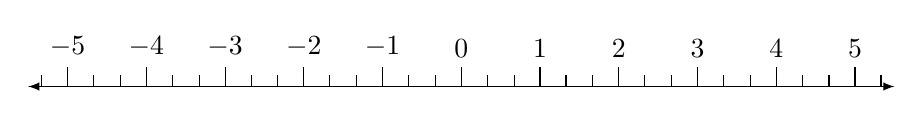
\begin{tikzpicture}
\draw[latex-latex] (-5.5, 0) -- (5.5, 0) ; 
\foreach \x in {-5,-4,-3,-2,-1,0,1,2,3,4,5} \draw (\x, 0) -- (\x, 0.25) node[above] {$\x$} ;
\foreach \x in {-5,-4,-3,-2,-1,0,1,2,3,4,5} {
  \foreach \i in {-0.33,0.33} {
    \draw (\x+\i, 0) -- (\x+\i, 0.15) ;
  }
}
\end{tikzpicture}
\end{center}
The rational numbers are those of the form $\frac{a}{b}$, where $a,b \in \mathbb{Z}$ and $b \ne 0$. We write $\mathbb{Q}$ \inlatex{mathbb\{Q\}}\lindexmmc{mathbb}{$\mathbb{A}, \mathbb{B}, \dots$} for the set of all rational numbers; thus, the notation `$q \in \mathbb{Q}$' means that $q$ is a rational number.
\end{definition}

The rational numbers are a very important example of a type of algebraic structure known as a \textit{field}---they are particularly central to algebraic number theory and algebraic geometry.

\subsection*{Real numbers ($\mathbb{R}$)}

Quantity and change can be measured in the abstract using \textit{real numbers}.

\begin{definition}
\label{defRealsInformal}
The \textbf{real numbers} are the points on the number line. We write $\mathbb{R}$ \inlatex{mathbb\{R\}}\lindexmmc{mathbb}{$\mathbb{A}, \mathbb{B}, \dots$} for the set of all real numbers; thus, the notation `$a \in \mathbb{R}$' means that $a$ is a real number.
\end{definition}

The real numbers are central to real analysis, a branch of mathematics introduced in \Cref{chRealNumbers}. They turn the rationals into a \textit{continuum} by `filling in the gaps'---specifically, they have the property of \textit{completeness}, meaning that if a quantity can be approximated with arbitrary precision by real numbers, then that quantity is itself a real number.

We can define the basic arithmetic operations (addition, subtraction, multiplication and division) on the real numbers, and a notion of ordering of the real numbers, in terms of the infinite number line.

\begin{itemize}
\item \textbf{Ordering.} A real number $a$ is less than a real number $b$, written $a<b$, if $a$ lies to the left of $b$ on the number line. The usual conventions for the symbols $\le$ \inlatex{le}\lindexmmc{le}{$\le$}, $>$ and $\ge$ \inlatex{ge}\lindexmmc{ge}{$\ge$} apply, for instance `$a \le b$' means that either $a < b$ or $a = b$.

\item \textbf{Addition.} Suppose we want to add a real number $a$ to a real number $b$. To do this, we \textit{translate} $a$ by $b$ units to the right---if $b<0$ then this amounts to translating $a$ by an equivalent number of units to the left. Concretely, take two copies of the number line, one above the other, with the same choice of unit length; move the $0$ of the lower number line beneath the point $a$ of the upper number line. Then $a+b$ is the point on the upper number line lying above the point $b$ of the lower number line.

Here is an illustration of the fact that $(-3) + 5 = 2$:

\begin{center}
\fitwidthc{0.9}{\begin{tikzpicture}
% Adapted from http://tex.stackexchange.com/questions/148252/
\draw[latex-latex] (-8.5,0) -- (5.5,0) ; 
\foreach \x in  {-8,-7,-6,-5,-4,-3,-2,-1,0,1,2,3,4,5}
\draw[shift={(\x,0)}] (0pt,3pt) -- (0pt,-3pt);
\foreach \x in {-8,-7,-6,-5,-4,-3,-2,-1,0,1,2,3,4,5}
\draw[shift={(\x,0)}] (0pt,0pt) -- (0pt,3pt) node[above] {$\x$};
\draw[*-*] (-3.08,0) -- (2.08,0);
\draw[very thick] (-3,0) -- (2,0);

\draw[latex-latex] (-8.5,-1) -- (5.5,-1) ; 
\foreach \x in  {-5,-4,-3,-2,-1,0,1,2,3,4,5,6,7,8}
\draw[shift={(\x-3,-1)},color=black] (0pt,3pt) -- (0pt,-3pt);
\foreach \x in {-5,-4,-3,-2,-1,0,1,2,3,4,5,6,7,8}
\draw[shift={(\x-3,-1)},color=black] (0pt,0pt) -- (0pt,-3pt) node[below] {$\x$};
\draw[dashed] (-3,-1) -- (-3,0) ;
\draw[->] (2,-0.8) -- (2,-0.2) ;
\end{tikzpicture}}
\end{center}

\item \textbf{Multiplication.} This one is fun. Suppose we want to multiply a real number $a$ by a real number $b$. To do this, we \textit{scale} the number line, and perhaps \textit{reflect} it. Concretely, take two copies of the number line, one above the other; align the $0$ points on both number lines, and stretch the lower number line evenly until the point $1$ on the lower number line is below the point $a$ on the upper number line---note that if $a<0$ then the number line must be reflected in order for this to happen. Then $a \cdot b$ is the point on the upper number line lying above $b$ on the lower number line.

Here is an illustration of the fact that $5 \cdot 4 = 20$.

\begin{center}
\fitwidthc{0.9}{\begin{tikzpicture}
% Adapted from http://tex.stackexchange.com/questions/148252/
\draw[latex-latex] (-5.5,0) -- (8.5,0) ; 
\foreach \x in  {-2,-1,0,1,2,3,4,5,6,7,8,9,10,11,12,13,14,15,16,17,18,19,20,21,22,23,24}
\draw[shift={(0.5*\x-4,0)}] (0pt,3pt) -- (0pt,-3pt);
\foreach \x in {-2,-1,0,1,2,3,4,5,6,7,8,9,10,11,12,13,14,15,16,17,18,19,20,21,22,23,24}
\draw[shift={(0.5*\x-4,0)}] (0pt,0pt) -- (0pt,3pt) node[above] {$\text{\footnotesize\x}$};
\draw[*-*] (-1.58,0) -- (6.08,0);
\draw[very thick] (-1.5,0) -- (6,0);

\draw[latex-latex] (-5.5,-1) -- (8.5,-1) ; 
\foreach \x in  {0,1,2,3,4}
\draw[shift={(2.5*\x-4,-1)},color=black] (0pt,3pt) -- (0pt,-3pt);
\foreach \x in {0,1,2,3,4}
\draw[shift={(2.5*\x-4,-1)},color=black] (0pt,0pt) -- (0pt,-3pt) node[below] {$\x$};
\draw[dashed] (-4,-1) -- (-4,0) ;
\draw[dashed] (-1.5,-1) -- (-1.5,0) ;
\draw[->] (6,-0.8) -- (6,-0.2) ;
\end{tikzpicture}}
\end{center}

and here is an illustration of the fact that $(-5) \cdot 4 = -20$:
\begin{center}
\fitwidthc{0.9}{\begin{tikzpicture}
% Adapted from http://tex.stackexchange.com/questions/148252/
\draw[latex-latex] (-5.5,0) -- (8.5,0) ; 
\foreach \x in  {-22,-21,...,4}
\draw[shift={(0.5*\x+6,0)}] (0pt,3pt) -- (0pt,-3pt);
\foreach \x in {-22,-21,...,4}
\draw[shift={(0.5*\x+6,0)}] (0pt,0pt) -- (0pt,3pt) node[above] {$\text{\footnotesize\x}$};
\draw[*-*] (-4.08,0) -- (3.58,0);
\draw[very thick] (-4,0) -- (3.5,0);

\draw[latex-latex] (-5.5,-1) -- (8.5,-1) ; 
\foreach \x in  {0,1,2,3,4}
\draw[shift={(6-2.5*\x,-1)},color=black] (0pt,3pt) -- (0pt,-3pt);
\foreach \x in {0,1,2,3,4}
\draw[shift={(6-2.5*\x,-1)},color=black] (0pt,0pt) -- (0pt,-3pt) node[below] {$\x$};
\draw[dashed] (6,-1) -- (6,0) ;
\draw[dashed] (3.5,-1) -- (3.5,0) ;
\draw[->] (-4,-0.8) -- (-4,-0.2) ;
\end{tikzpicture}}
\end{center}
\end{itemize}

\begin{exercise}
Interpret the operations of subtraction and division as geometric transformations of the real number line.
\end{exercise}

We will take for granted the arithmetic properties of the real numbers in this chapter, waiting until \Cref{secInequalitiesMeans} to sink our teeth into the details. For example, we will take for granted the basic properties of rational numbers, for instance
\[ \frac{a}{b}+\frac{c}{d} = \frac{ad+bc}{bd} \quad \text{and} \quad \frac{a}{b} \cdot \frac{c}{d} = \frac{ac}{bd} \]

\subsection*{Rational and irrational numbers}
\label{pGettingStartedRationalNumbers}

Before we can talk about irrational numbers, we should say what they are.

\begin{definition}
\label{defIrrationalNumber}
\index{irrational number}
An \textbf{irrational number} is a real number that is not rational.
\end{definition}

Unlike $\mathbb{N},\mathbb{Z},\mathbb{Q},\mathbb{R},\mathbb{C}$, there is no standard single letter expressing the irrational numbers. However, by the end of \Cref{secSetOperations}, we will be able to write the set of irrational numbers as $\mathbb{R} \setminus \mathbb{Q}$.

Note in particular that `irrational' does not simply mean `not rational'---that would imply that all complex numbers which are not real are irrational---rather, the term `irrational' means `real and not rational'.

Proving that a real number is \textit{irrational} is not particularly easy. We will get our foot in the door by allowing ourselves to assume the following result, which is restated and proved in \Cref{propSqrt2Irrational}.

\begin{proposition}
\label{propSqrt2IrrationalPreliminary}
The real number $\sqrt{2}$ is irrational. \qed
\end{proposition}

We can use the fact that $\sqrt{2}$ is irrational to prove some facts about the relationship between rational numbers and irrational numbers.

\begin{proposition}
Let $a$ and $b$ be irrational numbers. It is possible that $ab$ be rational.
\end{proposition}

\begin{cproof}
Let $a=b=\sqrt{2}$. Then $a$ and $b$ are irrational, and $ab=2=\frac{2}{1}$, which is rational.
\end{cproof}

\begin{exercise}
Let $r$ be a rational number and let $a$ be an irrational number. Prove that it is possible that $ra$ be rational, and it is possible that $ra$ be irrational.
\end{exercise}

\subsection*{Complex numbers ($\mathbb{C}$)}

We have seen that multiplication by real numbers corresponds with scaling and reflection of the number line---scaling alone when the multiplicand is positive, and scaling with reflection when it is negative. We could alternatively interpret this reflection as a \textit{rotation} by half a turn, since the effect on the number line is the same. You might then wonder what happens if we rotate by arbitrary angles, rather than only half turns.

What we end up with is a \textit{plane} of numbers, not merely a line---see \Cref{figComplexNumbers}. Moreover, it happens that the rules that we expect arithmetic operations to satisfy still hold---addition corresponds with translation, and multiplication corresponds with scaling and rotation. This resulting number set is that of the \textit{complex numbers}.

\begin{definition}
\label{defComplexNumbersInformal}
The \textbf{complex numbers} are those obtained by the non-negative real numbers upon rotation by any angle about the point $0$. We write $\mathbb{C}$ \inlatex{mathbb\{C\}}\lindexmmc{mathbb}{$\mathbb{A}, \mathbb{B}, \dots$} for the set of all complex numbers; thus, the notation `$z \in \mathbb{C}$' means that $z$ is a complex number.
\end{definition}

\begin{figure}[p!]
\centering
\resizebox{\textwidth}{!}{
\begin{tikzpicture}
\draw[latex-latex] (-5.5,0) -- (5.5,0) ;
\draw[latex-latex, dotted] (-4.76, 2.75) -- (4.76, -2.75) ;
\draw[latex-latex, dotted] (-2.75, 4.76) -- (2.75, -4.76) ;
\draw[latex-latex, dotted] (0, -5.5) -- (0, 5.5) ;
\draw[latex-latex, dotted] (2.75, 4.76) -- (-2.75, -4.76) ;
\draw[latex-latex, dotted] (4.76, 2.75) -- (-4.76, -2.75) ;
\draw[dotted] (0,0) circle [radius=1] ;
\draw[dotted] (0,0) circle [radius=2] ;
\draw[dotted] (0,0) circle [radius=3] ;
\draw[dotted] (0,0) circle [radius=4] ;
\draw[dotted] (0,0) circle [radius=5] ;
\foreach \x in  {-5,-4,-3,-2,-1,0,1,2,3,4,5}
  \draw[shift={(\x,0)}] (0pt,3pt) -- (0pt,-3pt);
\foreach \x in {-5,-4,-3,-2,-1,0,1,2,3,4,5}
  \draw[shift={(\x,0)}] (0,0) node[below right] {$\text{\small\x}$};
\draw (0,1) node[above right] {$i$};
\draw (-3pt,1) -- (3pt,1);
\foreach \x in {2,3,4,5}
  \draw[shift={(0,\x)}] (0,0) node[above right] {$\x i$};
\foreach \x in {2,3,4,5}
  \draw[shift={(0,\x)}] (-3pt,0pt) -- (3pt, 0pt);
\foreach \x in {2,3,4,5}
  \draw[shift={(0,-\x)}] (0,0) node[below right] {$\text{\small-}\x i$};
\foreach \x in {2,3,4,5}
  \draw[shift={(0,-\x)}] (-3pt,0pt) -- (3pt, 0pt);
\draw (0,-1) node[below right] {$\text{\small-}i$};
\draw (-3pt,-1) -- (3pt,-1);
\end{tikzpicture}
}
\caption{Illustration of the complex plane, with some points labelled.}
\label{figComplexNumbers}
\end{figure}

There is a particularly important complex number, $i$, which is the point in the complex plane exactly one unit above $0$---this is illustrated in \Cref{figComplexNumbers}. Multiplication by $i$ has the effect of rotating the plane by a quarter turn anticlockwise. In particular, we have $i^2 = i \cdot i = -1$; the complex numbers have the astonishing property that square roots of \textit{all} complex numbers exist (including all the real numbers).

In fact, every complex number can be written in the form $a+bi$, where $a,b \in \mathbb{R}$; this number corresponds with the point on the complex plane obtained by moving $a$ units to the right and $b$ units up, reversing directions as usual if $a$ or $b$ is negative. Arithmetic on the complex numbers works just as with the real numbers; in particular, using the fact that $i^2=-1$, we obtain
\[ (a+bi)+(c+di) = (a+c)+(b+d)i \quad \text{and} \quad (a+bi) \cdot (c+di) = (ac-bd) + (ad+bc)i \]

We will discuss complex numbers further in the portion of this chapter on polynomials below.

\subsection*{Polynomials}
\label{pGettingStartedPolynomials}

The integers, rational numbers, real numbers and complex numbers are all examples of \textit{rings}, which means that they come equipped with nicely behaving notions of addition, subtraction and multiplication.

\begin{definition}
\label{defPolynomialPreliminary}
\index{polynomial}
Let $A$ be one $\mathbb{Z}$, $\mathbb{Q}$, $\mathbb{R}$ or $\mathbb{C}$. A (\textbf{univariate}) \textbf{polynomial over $A$} in the \textbf{indeterminate} $x$ is an expression of the form
\[ a_0 + a_1x + \cdots + a_nx^n \]
where $n \in \mathbb{N}$ and each $a_k \in A$. The numbers $a_k$ are called the \textbf{coefficients} of the polynomial. If not all coefficients are zero, the largest value of $k$ for which $a_k \ne 0$ is called the \textbf{degree} of the polynomial. By convention, the degree of the polynomial $0$ is $-\infty$.
\end{definition}

Polynomials of degree $1$, $2$, $3$, $4$ and $5$ are respectively called \textit{linear}, \textit{quadratic}, \textit{cubic}, \textit{quartic} and \textit{quintic} polynomials.

\begin{example}
The following expressions are all polynomials:
\[ 3 \qquad 2x-1 \qquad (3+i)x^2-x \]
Their degrees are $0$, $1$ and $2$, respectively. The first two are polynomials over $\mathbb{Z}$, and the third is a polynomial over $\mathbb{C}$.
\end{example}

\begin{exercise}
Write down a polynomial of degree $4$ over $\mathbb{R}$ which is not a polynomial over $\mathbb{Q}$.
\end{exercise}

\begin{notation}
Instead of writing out the coefficients of a polynomial each time, we may write something like $p(x)$ or $q(x)$. The `$(x)$' indicates that $x$ is the indeterminate of the polynomial. If $\alpha$ is a number\footnote{When dealing with polynomials, we will typically reserve the letter $x$ for the indeterminate variable, and use the Greek letters $\alpha,\beta,\gamma$ \inlatex{alpha, \textbackslash{}beta, \textbackslash{}gamma} for numbers to be substituted into a polynomial.} and $p(x)$ is a polynomial in indeterminate $x$, we write $p(\alpha)$ for the result of \textbf{substituting} $\alpha$ for $x$ in the expression $p(x)$.
\end{notation}

Note that, if $A$ is any of the sets $\mathbb{N}$, $\mathbb{Z}$, $\mathbb{Q}$, $\mathbb{R}$ or $\mathbb{C}$, and $p(x)$ is a polynomial over $A$, then $p(\alpha) \in A$ for all $\alpha \in A$.

\begin{example}
Let $p(x)=x^3-3x^2+3x-1$. Then $p(x)$ is a polynomial over $\mathbb{Z}$ with indeterminate $x$. For any integer $\alpha$, the value $p(\alpha)$ will also be an integer. For example
\[ p(0) = 0^3-3 \cdot 0^2 + 3 \cdot 0 - 1 = -1 \quad \text{and} \quad p(3) = 3^3 - 3 \cdot 3^2 + 3 \cdot 3 - 1 = 8 \]
\end{example}

\begin{definition}
\label{defRootOfPolynomial}
\index{root}
Let $p(x)$ be a polynomial. A \textbf{root} of $p(x)$ is a complex number $\alpha$ such that $p(\alpha)=0$.
\end{definition}

The \textit{quadratic formula} (\Cref{thmQuadraticFormula}) tells us that the roots of the polynomial $x^2+ax+b$, where $a,b \in \mathbb{C}$, are precisely the complex numbers
\[ \frac{-a+\sqrt{a^2-4b}}{2} \quad \text{and} \quad \frac{-a-\sqrt{a^2-4b}}{2} \]

Note our avoidance of the symbol `$\pm$', which is commonly found in discussions of quadratic polynomials. The symbol `$\pm$' is dangerous because it may suppress the word `and' or the word `or', depending on context---this kind of ambiguity is not something that we will want to deal with when discussing the logical structure of a proposition in \Cref{chLogicalStructure}!

\begin{example}
\label{exApplicationOfQuadraticFormula}
Let $p(x)=x^2-2x+5$. The quadratic formula tells us that the roots of $p$ are
\begin{center}
$\dfrac{2 + \sqrt{4 - 4 \cdot 5}}{2} = 1 + \sqrt{-4} = 1+2i$
\quad and \quad
$\dfrac{2 - \sqrt{4 - 4 \cdot 5}}{2} = 1-\sqrt{-4} = 1-2i$
\end{center}
The numbers $1+2i$ and $1-2i$ are related in that their real parts are equal and their imaginary parts differ only by a sign. \Cref{exComplexNumberAsRootOfQuadraticOverR} generalises this observation.
\end{example}

\begin{exercise}
\label{exComplexNumberAsRootOfQuadraticOverR}
Let $\alpha = a+bi$ be a complex number, where $a,b \in \mathbb{R}$. Prove that $\alpha$ is the root of a quadratic polynomial over $\mathbb{R}$, and find the other root of this polynomial.
\end{exercise}

The following exercise proves the well-known result which classifies the number of real roots of a polynomial over $\mathbb{R}$ in terms of its coefficients.

\begin{exercise}
\label{exDiscriminantRealRoots}
\index{discriminant}
Let $a,b \in \mathbb{C}$ and let $p(x)=x^2+ax+b$. The value $\Delta=a^2-4b$ is called the \textbf{discriminant} of $p$. Prove that $p$ has two roots if $\Delta \ne 0$ and one root if $\Delta = 0$. Moreover, if $a,b \in \mathbb{R}$, prove that $p$ has no real roots if $\Delta < 0$, one real root if $\Delta = 0$, and two real roots if $\Delta > 0$.
\end{exercise}

\begin{example}
Consider the polynomial $x^2-2x+5$. Its discriminant is equal to $(-2)^2-4 \cdot 5 = -16$, which is negative. \Cref{exDiscriminantRealRoots} tells us that it has two roots, neither of which are real. This was verified by \Cref{exApplicationOfQuadraticFormula}, where we found that the roots of $x^2-2x+5$ are $1+2i$ and $1-2i$.

Now consider the polynomial $x^2-2x-3$. Its discriminant is equal to $(-2)^2-4\cdot(-3) = 16$, which is positive. \Cref{exDiscriminantRealRoots} tells us that it has two roots, both of which are real; and indeed
\[ x^2-2x-3 = (x+1)(x-3) \]
so the roots of $x^2-2x-3$ are $-1$ and $3$.
\end{example}